\section{Analisi del problema}
Uno dei principali problemi che le organizzazioni si trovano ad affrontare riguarda la capacità di \textbf{individuare tempestivamente attività malevole} all'interno dei propri sistemi.  
La sicurezza informatica rappresenta oggi una delle sfide più complesse per le aziende di qualsiasi settore. Le infrastrutture \textit{IT} moderne sono caratterizzate da un'elevata interconnessione e da una crescente dipendenza da servizi digitali, fattori che le rendono esposte a minacce sempre più sofisticate. Gli attacchi informatici non sono più episodi sporadici, ma eventi ricorrenti che possono compromettere la continuità operativa, causare perdite economiche e danneggiare in modo significativo l'azienda.\\
Le tecniche di attacco evolvono rapidamente e gli strumenti difensivi tradizionali, come \textit{firewall} e \textit{antivirus}, non sempre riescono a garantire una protezione completa. Gli operatori malevoli, infatti, sfruttano vulnerabilità sconosciute, configurazioni errate o semplicemente il fattore umano, riuscendo così ad aggirare i controlli di sicurezza.\\  
A ciò si aggiunge la difficoltà di comprendere a fondo il comportamento degli attaccanti. Spesso le aziende hanno una visibilità limitata su quali metodi vengano impiegati, su come gli aggressori si muovano una volta ottenuto l'accesso e su quali siano gli obiettivi finali delle intrusioni. Questa mancanza di informazioni rende complesso elaborare strategie di difesa realmente efficaci e impedisce di anticipare possibili minacce future.\\
In sintesi, il problema principale è legato all'\textbf{assenza di strumenti e metodologie} che consentano non solo di rilevare gli attacchi, ma anche di comprenderne le dinamiche e trarne conoscenza utile per migliorare la sicurezza complessiva dei sistemi informativi.
\begin{figure}[H]
    \begin{center}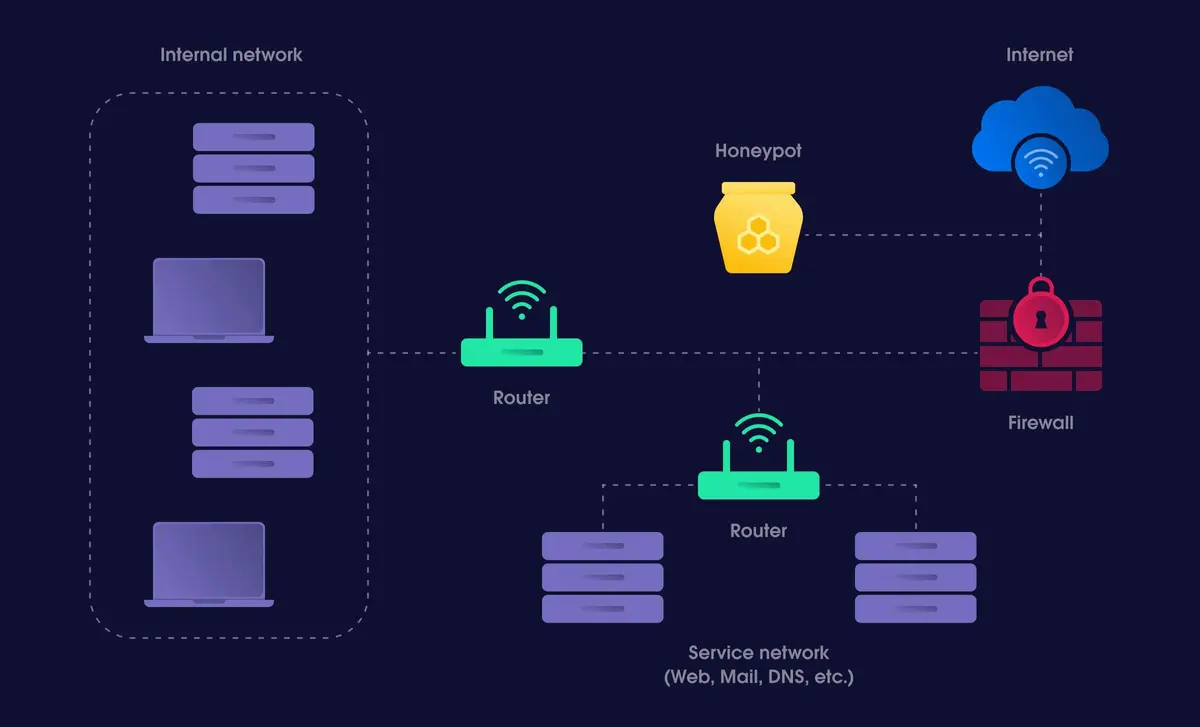
\includegraphics[alt={Honeypot position}, width=\columnwidth]{img/honeypot.jpg}
    \caption{Esempio di utilizzo di un sistema \textit{honeypot}.}
    Fonte: \url{https://oxylabs.io/blog/what-is-a-honeypot}
    \end{center}
\end{figure}
\label{fig:honeypot}